\documentclass{beamer}

% For more themes, color themes and font themes, see:
% http://deic.uab.es/~iblanes/beamer_gallery/index_by_theme.html
%
\mode<presentation>
{
  \usetheme{Madrid}       % or try default, Darmstadt, Warsaw, ...
  \usecolortheme{default} % or try albatross, beaver, crane, ...
  \usefonttheme{serif}    % or try default, structurebold, ...
  \setbeamertemplate{navigation symbols}{}
  \setbeamertemplate{caption}[numbered]
} 

\usepackage{tikz}
\usetikzlibrary{decorations.markings,angles}
\usepackage{tikz-3dplot} 

\usepackage{amsmath}


\begin{document}

\newcommand{\tikzAngleOfLine}{\tikz@AngleOfLine}
  \def\tikz@AngleOfLine(#1)(#2)#3{%
  \pgfmathanglebetweenpoints{%
    \pgfpointanchor{#1}{center}}{%
    \pgfpointanchor{#2}{center}}
  \pgfmathsetmacro{#3}{\pgfmathresult}%
  }



\begin{frame}{Geometric representation}
Radiation of a non relativistic charge accelelerated free or bound 
(electron in the classical description with oscillators) 


\begin{equation}
	\vec{E_{rad}} \propto  \vec{n} \times (\vec{n} \times \vec{a}) 
\end{equation}



\end{frame}

\begin{frame}{Geometric representation}
Electron accelerated by a  force due to the electric field of polarized radiation 
(Thomson scattering)
\tdplotsetmaincoords{60}{120} 
\begin{tikzpicture} [scale=2, tdplot_main_coords, 
axis/.style={->, thick},
osc/.style={ blue, very thick},
vector/.style={<->,red,very thick}]

%standard tikz coordinate definition using x, y, z coords

%tikz-3dplot coordinate definition using x, y, z coords


\node[tdplot_main_coords,anchor=south east] at (0,2,0){O};

%\coordinate (y1) at (1.5,3.5);
\coordinate (y1) at (1.38,3.12);
\coordinate (y2) at (1.12,3.38);

\coordinate (x1) at (-0.5,0,0);
\coordinate (x2) at (0.5,0,0);

\coordinate (y11) at (0,2,-0.5);
\coordinate (y12) at (0,2,0.5);
\coordinate (x11) at (-0.5,2,0);
\coordinate (x12) at (0.5,2,0);
\coordinate (z1) at (0,1.5,0);
\coordinate (z2) at (0,2.5,0);

\coordinate (y21) at (2,2,-0.5);
\coordinate (y22) at (2,2,0.5);

\coordinate (O1) at (0,0,0);
\coordinate (O) at (0,2,0);


%draw axes
\draw[axis] (-1,2,0) -- (3,2,0) node[anchor=north east]{$x$};
\draw[axis] (0,-1,0) -- (0,3,0) node[anchor=north west]{$y$};
\draw[axis] (-1,1,0) -- (2,4,0) node[anchor=north west]{$n$};
\draw[axis] (-1,3,0) -- (1,1,0) node[anchor=north west]{$x'$};
\draw[axis] (0,2,-1) -- (0,2,1) node[anchor=south]{$z$};

\coordinate (A) at (0.5,2.5,0); %n 
\coordinate (B) at (0.5,2,0); 


    \tikzAngleOfLine(O)(B){\AngleEnd}
    \tikzAngleOfLine(O)(A){\AngleStart}
    \draw[<->] (A)+(\AngleStart:0.3cm) arc (\AngleStart:\AngleEnd:0.7 cm);
    \node at ($(A)+({(\AngleStart+\AngleEnd)/2}:.4 cm)$) {$\alpha$};



%draw a vector from O to P
\draw[vector] (x1) -- (x2);
\draw[vector] (y1) -- (y2);

\draw[osc] (x11) -- (x12);
\draw[osc] (y11) -- (y12);
\draw[osc] (z1) -- (z2);


\end{tikzpicture}

$\vec{x},\vec{y},\vec{n},\vec{x'}$  same plane

\end{frame}

\begin{frame}{Geometric representation}
\begin{itemize}
\item Anisotropic radiation creates a net dipole moment in scattering atoms or molecules
(Rayleigh scattering) 
\item shorter wavelengths more scattered 	
\end{itemize}
\end{frame}

\begin{frame}{Geometric representation}
Incident unpolarized light, cartesian oscillators
\tdplotsetmaincoords{60}{120} 
\begin{tikzpicture} [scale=2, tdplot_main_coords, 
axis/.style={->, thick},
osc/.style={ blue, very thick},
vector/.style={<->,red,very thick}]

%standard tikz coordinate definition using x, y, z coords

%tikz-3dplot coordinate definition using x, y, z coords


\node[tdplot_main_coords,anchor=south east] at (0,2,0){O};

\coordinate (y1) at (0,0,-0.5);
\coordinate (y2) at (0,0,0.5);
\coordinate (x1) at (-0.5,0,0);
\coordinate (x2) at (0.5,0,0);

\coordinate (y11) at (0,2,-0.5);
\coordinate (y12) at (0,2,0.5);
\coordinate (x11) at (-0.5,2,0);
\coordinate (x12) at (0.5,2,0);
\coordinate (z1) at (0,1.5,0);
\coordinate (z2) at (0,2.5,0);

\coordinate (y21) at (2,2,-0.5);
\coordinate (y22) at (2,2,0.5);

\coordinate (O1) at (0,0,0);
\coordinate (O) at (0,2,0);


%draw axes
\draw[axis] (-1,2,0) -- (3,2,0) node[anchor=north east]{$x$};
\draw[axis] (0,-1,0) -- (0,3,0) node[anchor=north west]{$y$};
\draw[axis] (0,2,-1) -- (0,2,1) node[anchor=south]{$z$};

%draw a vector from O to P
\draw[vector] (x1) -- (x2);
\draw[vector] (y1) -- (y2);

\draw[osc] (x11) -- (x12);
\draw[osc] (y11) -- (y12);
\draw[osc] (z1) -- (z2);

\draw[vector] (y21) -- (y22);

\end{tikzpicture}

\end{frame}

\begin{frame}{Geometric representation}
Incident unpolarized light, circular oscillators
\tdplotsetmaincoords{60}{120} 
\begin{tikzpicture} [scale=2, tdplot_main_coords, 
axis/.style={->, thick},
osc/.style={ blue, very thick   },
vector/.style={<->,red,very thick}]

%standard tikz coordinate definition using x, y, z coords

%tikz-3dplot coordinate definition using x, y, z coords


\node[tdplot_main_coords,anchor=south east] at (0,2,0){O};

\coordinate (y1) at (0,0,-0.5);
\coordinate (y2) at (0,0,0.5);
\coordinate (x1) at (-0.5,0,0);
\coordinate (x2) at (0.5,0,0);

\coordinate (x11) at (-0.5,2,0);
\coordinate (x12) at (0.5,2,0);
\coordinate (c1) at (0.1,2,0);
\coordinate (c2) at (-0.1,2,0);


\coordinate (y21) at (2,2,-0.5);
\coordinate (y22) at (2,2,0.5);

\coordinate (O1) at (0,0,0);
\coordinate (O) at (0,2,0);


%draw axes
\draw[axis] (-1,2,0) -- (3,2,0) node[anchor=north east]{$x$};
\draw[axis] (0,-1,0) -- (0,3,0) node[anchor=north west]{$y$};
\draw[axis] (0,2,-1) -- (0,2,1) node[anchor=south]{$z$};

%draw a vector from O to P
\draw[vector] (x1) -- (x2);
\draw[vector] (y1) -- (y2);

\draw[osc] (x11) -- (x12);
\draw[osc,decoration={markings, mark=at position 0.2 with {\arrow{<}}},
        postaction={decorate}] (c1) circle (0.5cm);
\draw[osc,decoration={markings, mark=at position 0.2 with {\arrow{>}}},
        postaction={decorate}] (c2) circle (0.5cm);

\draw[vector] (y21) -- (y22);

\end{tikzpicture}
coherence between circular oscillators
\end{frame}

\begin{frame}{Geometric representation}
Magnetic field along l.o.s , circular oscillators 
\tdplotsetmaincoords{60}{120} 
\begin{tikzpicture} [scale=2, tdplot_main_coords, 
axis/.style={->, thick},
osc/.style={ blue, very thick   },
vector/.style={<->,red,very thick}]

%standard tikz coordinate definition using x, y, z coords

%tikz-3dplot coordinate definition using x, y, z coords


\node[tdplot_main_coords,anchor=south east] at (0,0,0){O};


\coordinate (x11) at (-0.5,0,0);
\coordinate (x12) at (0.5,0,0);
\coordinate (c1) at (0.1,0,0);
\coordinate (c2) at (-0.1,0,0);


\coordinate (y2) at (2,0,0);

\coordinate (O) at (0,2,0);


%draw axes
\draw[axis] (-1,0,0) -- (3,0,0) node[anchor=north east]{$x$};
\draw[axis] (0,-1,0) -- (0,1,0) node[anchor=north west]{$y$};
\draw[axis] (0,0,-1) -- (0,0,1) node[anchor=south]{$z$};
\draw[axis] (2,0,-1) -- (2,0,1) node[anchor=south]{$$};

%draw a vector from O to P

\draw[osc] (x11) -- (x12);
\draw[osc,decoration={markings, mark=at position 0.2 with {\arrow{<}}},
        postaction={decorate}] (c1) circle (0.5cm);
\draw[osc,decoration={markings, mark=at position 0.2 with {\arrow{>}}},
        postaction={decorate}] (c2) circle (0.5cm);
\draw[red, very thick,decoration={markings, mark=at position 0.2 with {\arrow{>}}},
        postaction={decorate}] (y2) circle (0.5cm);

\draw[->, very thick] (0.5,1.25,0) -- (2,1.25,0);
\node at (2,1.25,0)[anchor=north]{$\vec{B}$};

\end{tikzpicture}
ciclotron radiation
\end{frame}
\begin{frame}{Geometric representation}
Unpolarized incident light and magnetic field along l.o.s , circular oscillators
\begin{figure}[H]
 \centering
 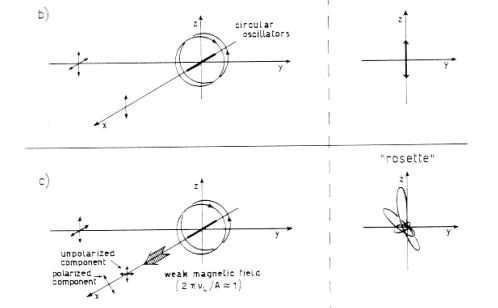
\includegraphics[scale=0.5]{a2.png}
  \caption{Incoherence in the circular oscillators - Hanle effect}
\end{figure}
\end{frame}


\begin{frame}{Quantic representation (bound electron)}
\begin{figure}[H]
 \centering
 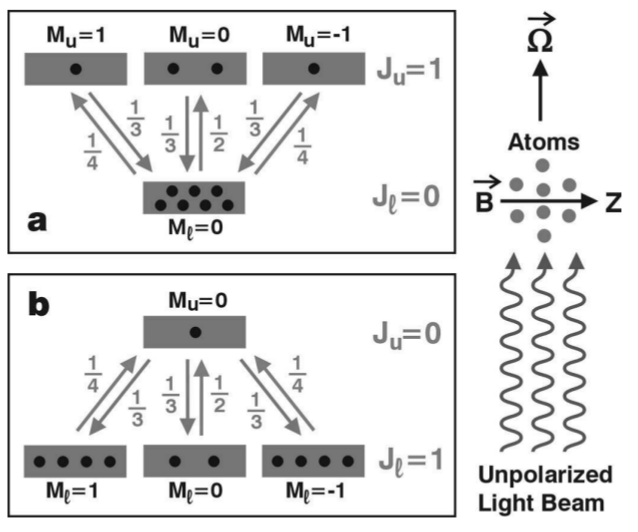
\includegraphics[scale=0.5]{a1.png}
  \caption{Emission/Absorption}
\end{figure}
\end{frame}

\begin{frame}{Quantic representation (bound electron)}
\begin{itemize}
\item Correspondence between atomic transitions and radiation components
\begin{itemize}
\item $\Delta M = 1$, $\sigma_+$ ($\nu + \nu_L$), clockwise oscillator
\item $\Delta M = 0$, $\pi$ ($\nu$), x oscillator
\item $\Delta M = -1$, $\sigma_-$ ($\nu - \nu_L$), anticlockwise oscillator
\end{itemize}
\item similar mechanism(Fig 2 b)  for absorption lines
(experimetally done by observing same line in filaments: absorption and in prominences: emission)
\item Anisotropic radiation populates/depopulates twice M=0 sublevel
\item Magnetic field:
\begin{itemize}

\item splitting of  energy level J into 2J+1 sublevels (Zeeman effect) 
\item creates incoherence between  population of levels corresponding  to $\sigma$ components which leads to
incoherence in the 2 circular oscillators (Hanle effect)


\end{itemize}
\end{itemize}

\end{frame}


\begin{frame}{Second specter of the sun}
With the same geometry: Q represents linear polarization parallel to the closest limb
\begin{figure}[H]
 \centering
 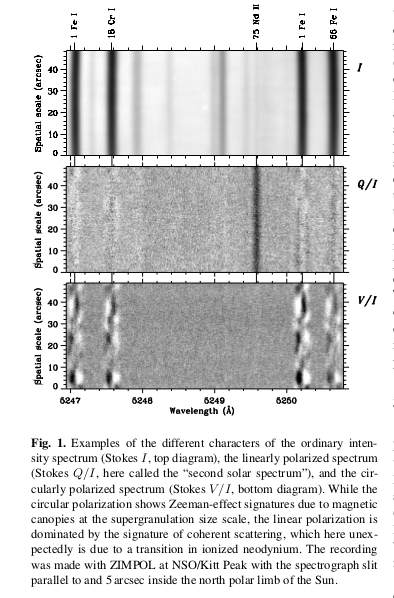
\includegraphics[scale=0.5]{a3.png}
\end{figure}
\end{frame}

\begin{frame}{Second specter of the sun}
Unknown I 0 level

Eliminating Q signal generated by other mechanisms

\begin{itemize}

\item atmospheric seeing and CCD noise: resolved by modulating the signal at high frequency: 2 modulators one
at 42 kHz and 84 kHz

\item position near the (geographic) north/south pole where influence of the magnetic field is smaller

\item cross talk Stokes V generated by the magnetic field recognized (sign reversed with spatial period = the size of a granulation)
which confirms the existence of horrizontal  magnetic field oriented along the line of sight 

\item vertical magnetic field 

\item horrizontal magnetic field perpendicular to line of sight

\item polarization by reflection
\end{itemize}
\end{frame}

\begin{frame}{Vertical magnetic field}
\tdplotsetmaincoords{60}{120} 
\begin{tikzpicture} [scale=2, tdplot_main_coords, 
axis/.style={->, thick},
osc/.style={ blue, very thick   },
vector/.style={<->,red,very thick}]

%standard tikz coordinate definition using x, y, z coords

%tikz-3dplot coordinate definition using x, y, z coords


\node[tdplot_main_coords,anchor=south east] at (0,2,0){O};

\coordinate (y1) at (0,0,-0.5);
\coordinate (y2) at (0,0,0.5);
\coordinate (x1) at (-0.5,0,0);
\coordinate (x2) at (0.5,0,0);

\coordinate (x11) at (-0.5,2,0);
\coordinate (x12) at (0.5,2,0);
\coordinate (y11) at (0,2,-0.5);
\coordinate (y12) at (0,2,0.5);
\coordinate (z1) at (0,1.5,0);
\coordinate (z2) at (0,2.5,0);

\coordinate (y21) at (2,2,-0.5);
\coordinate (y22) at (2,2,0.5);

\coordinate (O1) at (0,0,0);
\coordinate (O) at (0,2,0);


%draw axes
\draw[axis] (-1,2,0) -- (3,2,0) node[anchor=north east]{$x$};
\draw[axis] (0,-1,0) -- (0,3,0) node[anchor=north west]{$y$};
\draw[axis] (0,2,-1) -- (0,2,1) node[anchor=south]{$z$};

%draw a vector from O to P
\draw[vector] (x1) -- (x2);
\draw[vector] (y1) -- (y2);

\draw[osc] (x11) -- (x12);
\draw[osc] (y11) -- (y12);
\draw[osc] (z1) -- (z2);

\draw[->, very thick] (0.5,2.5,0) -- (0.5,3,0);
\node at (0.5,3,0)[anchor=north]{$\vec{B}$};
\draw[vector] (y21) -- (y22);

\end{tikzpicture}
 
effect adding to that of the radiation: linear polarization (no V signal, no Hanle effect)

\end{frame}

\begin{frame}{Horrizontal magnetic field, perpendicular to l.o.s. }
\tdplotsetmaincoords{60}{120} 
\begin{tikzpicture} [scale=2, tdplot_main_coords, 
axis/.style={->, thick},
osc/.style={ blue, very thick   },
vector/.style={<->,red,very thick}]

%standard tikz coordinate definition using x, y, z coords

%tikz-3dplot coordinate definition using x, y, z coords


\node[tdplot_main_coords,anchor=south east] at (0,2,0){O};

\coordinate (y1) at (0,0,-0.5);
\coordinate (y2) at (0,0,0.5);
\coordinate (x1) at (-0.5,0,0);
\coordinate (x2) at (0.5,0,0);

\coordinate (x11) at (-0.5,2,0);
\coordinate (x12) at (0.5,2,0);
\coordinate (y11) at (0,2,-0.5);
\coordinate (y12) at (0,2,0.5);
\coordinate (z1) at (0,1.5,0);
\coordinate (z2) at (0,2.5,0);

\coordinate (y21) at (2,2,-0.5);
\coordinate (y22) at (2,2,0.5);
\coordinate (y31) at (2,1.8,0);
\coordinate (y32) at (2,2.2,0);

\coordinate (O1) at (0,0,0);
\coordinate (O) at (0,2,0);


%draw axes
\draw[axis] (-1,2,0) -- (3,2,0) node[anchor=north east]{$x$};
\draw[axis] (0,-1,0) -- (0,3,0) node[anchor=north west]{$y$};
\draw[axis] (0,2,-1) -- (0,2,1) node[anchor=south]{$z$};

%draw a vector from O to P
\draw[vector] (x1) -- (x2);
\draw[vector] (y1) -- (y2);

\draw[osc] (x11) -- (x12);
\draw[osc] (y11) -- (y12);
\draw[osc] (z1) -- (z2);

\draw[->, very thick] (0,3.5,0) -- (0,3.5,1);
\node at (0,3.5,1)[anchor=south]{$\vec{B}$};
\draw[vector] (y21) -- (y22);
\draw[vector] (y31) -- (y32);

\end{tikzpicture}

horrizontal component(Hanle effect), no V signal
\end{frame}


\begin{frame}{Polarization by reflection}
	\begin{figure}[H]
 \centering
 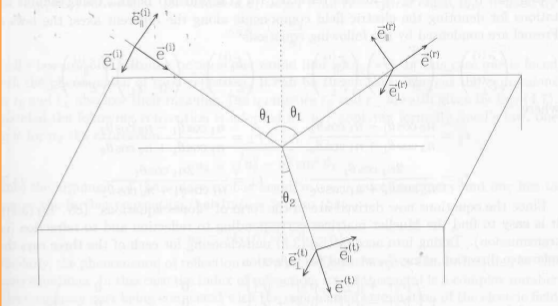
\includegraphics[scale=0.5]{a5.png}
\end{figure}
\end{frame}


\begin{frame}{Polarization by reflection}
\begin{figure}[H]
 \centering
 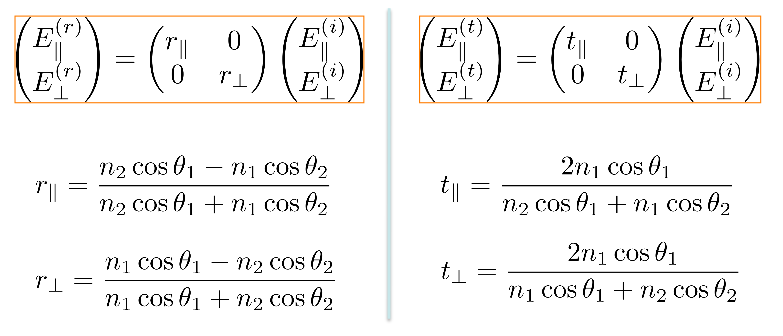
\includegraphics[scale=0.5]{a6.png}
\end{figure}
$n_1 = 1 < n_2, cos \theta_1 < cos \theta_2 \implies ( n_2 cos \theta_1 = cos \theta_2 \implies r_{\parallel} = 0) $

$sin \theta_1 = n_2 sin \theta_2 \implies 1 - (cos \theta_1)^2 = n_2^2 (1 - n_2^2 (cos \theta_1)^2) $

$ \theta_1 = arccos (\sqrt{\frac{n_2^2 -1}{n_2^4-1}}) \implies  $ reflected light polarized along $r_{\perp}$
\end{frame}
\begin{frame}{Observation details}
\begin{itemize}

\item instrument: ZIMPOL, the Zurich Imaging Stokes Polarimeter 
\item telescope: McMath-Pierce(National Solar Observatory (Kitt Peak, USA).)
\item accuracy: $10^{-5}$
\item April 1995, slit positioned 5 seconds of arc inside the north polar limb 
(where the cosine $\mu$ of the heliocentric angle is 0.1)
\end{itemize}
\end{frame}
\end{document}
